\documentclass[../main.tex]{subfiles}
\graphicspath{{\subfix{../images/}}}
\begin{document}

  Para o desenvolvimento do projeto, foi criada uma metodologia própria a ser seguida, composta por quatro fases sequenciais, conforme ilustrado na figura \ref{fig:metodologia} e detalhado a seguir. \textbf{\textcolor{red}{Colocar como apêndice?}}

  \begin{figure*}[h]
    \centering
    \caption{Metodologia}
    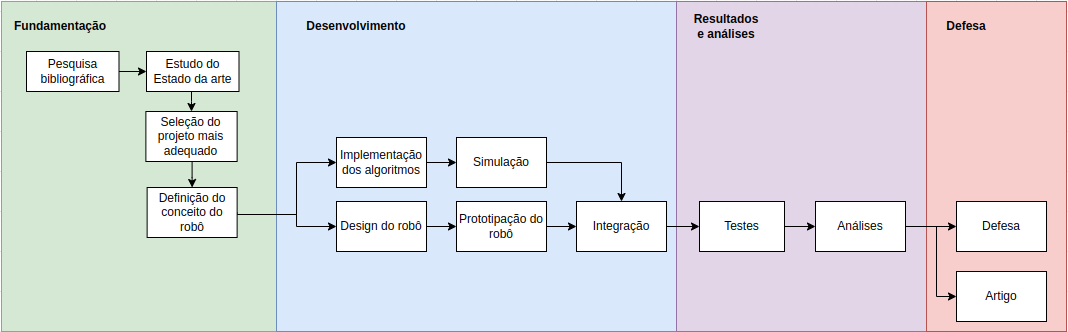
\includegraphics[width=\textwidth]{metodologia.png}

    Fonte: Proprio autor
    \label{fig:metodologia}
  \end{figure*}

  \subsection{Fundamentação}
  A primeira fase da metodologia tem como objetivo buscar referências que possam embasar o estudo e servir de padrão para o design e desenvolvimento do projeto.

  Durante essa fase de Fundamentação, o primeiro a ser feito são pesquisas bibliográficas, com o intuito de selecionar artigos úteis e correlatos ao projeto. \textcolor{red}{Para isso, foi utilizado o \textit{Método Bili}.}

  A partir dessas pesquisas, é possível realizar um Estudo do Estado da Arte, selecionando, a partir de um \textcolor{red}{Benchmarking} realizado com robôs quadrúpedes, projetos que possam servir de referência para o desenvolvimento, definindo os \textcolor{red}{conceitos, funcionalidades e design} que o projeto deverá ter.

  \subsection{Desenvolvimento}
  Durante esta etapa da metodologia, ocorre o desenvolvimento do robô propriamente dito. Inicialmente, duas etapas ocorrem de forma parelela, sendo elas a implementação e simulação dos algoritmos (em ambiente computacional) e a definição e prototipação do design do robô.

  Durante a implementação de algoritmos e simulação, são inicialmente elaborados o diagrama de blocos do sistema e a arquitetura de software do controlador, de forma a padronizar e documentar o desenvolvimento do projeto. A partir disso, os algoritmos de cinemática e controle podem ser implementados e testados em simulação. Para auxiliar e possibilitar o desenvolvimento do projeto, algumas ferramentas e \textit{Softwares} serão utilizados. O ROS - Robot Operating System é um conjunto de bibliotecas e ferramentas de \textit{software Open Source} que auxiliam no desenvolvimento de aplicações robóticas. O ROS Humble, nativo para Ubuntu 22.04, será utilizado, por possuir boa documentação e comunidade ativa, além de possuir pacotes muito úteis para o desenvolvimento do robô. 

  Em paralelo com o desenvolvimento de software, a prototipação e construção do robô é realizada, através da elaboração dos desenhos mecânicos e projetos eletro-eletrônicos. Esta etapa inclui também a impressão 3D das partes mecânicas projetadas, teste dos atuadores e sensores e configuração e comunicação entre o processador e os servo-motores Dynamixel \textcolor{red}{modelo?} que serão utilizados, culminando na montagem física do protótipo funcional. Os Softwares OnShape e XXXX serão utilizados para o desenvolvimento do CAD do robô e para seu projeto elétrico, respectivamente.

  Após essas etapas, é possível realizar a integração dos algoritmos no protótipo físico, de forma a validar o desenvolvimento realizado em ambiente computacional em um robô no mundo real.

  \subsection{Resultados e Análises}
  A etapa de resultados e análises tem como objetivo inicial realizar testes a fim de coletar dados para a análise de performance dos algoritmos implementados no robô. Durante essa etapa, será feita também uma analise comparativa entre os resultados obtidos em ambiente de simulação e no mundo real. \textcolor{red}{Detalhamento de quais testes serão feitos?}

  \subsection{Defesa}
  Esta é a última etapa da metodologia, que consiste na finalização e revisão do artigo e na apresentação de defesa do trabalho perante a banca avaliadora. 

\end{document}
